\documentclass[11pt,a4paper]{article}
\usepackage[utf8]{inputenc}
\usepackage[margin=1in]{geometry}
\usepackage{graphicx}
\usepackage{booktabs}
\usepackage{hyperref}
\usepackage{listings}
\usepackage{xcolor}
\usepackage{authblk}
\usepackage{pgfplots}
\pgfplotsset{width=10cm,compat=1.9}

\definecolor{codegreen}{rgb}{0,0.6,0}
\definecolor{codegray}{rgb}{0.5,0.5,0.5}
\definecolor{codepurple}{rgb}{0.58,0,0.82}
\definecolor{backcolour}{rgb}{0.95,0.95,0.92}

\lstdefinestyle{mystyle}{
backgroundcolor=\color{backcolour}, 
commentstyle=\color{codegreen},
keywordstyle=\color{magenta},
numberstyle=\tiny\color{codegray},
stringstyle=\color{codepurple},
basicstyle=\ttfamily\footnotesize,
breakatwhitespace=false, 
breaklines=true, 
captionpos=b, 
keepspaces=true, 
numbers=left, 
numbersep=5pt, 
showspaces=false, 
showstringspaces=false,
showtabs=false, 
tabsize=2
}

\lstset{style=mystyle}

\title{\textbf{RagCLI: A High-Performance Command Line Interface for\\Retrieval Augmented Generation with Oracle Database 23ai}}

\author{Nacho Martínez (jasperan)}
\affil{Data Scientist Advocate at Oracle \\ \url{https://github.com/jasperan}}

\date{\today}

\begin{document}

\maketitle

\begin{abstract}
I introduce \texttt{ragcli}, a full-featured, high-performance Command Line Interface (CLI) for Retrieval Augmented Generation (RAG). By utilizing the AI Vector Search capabilities within Oracle Database 23ai, combined with the highly-efficient Gemma 3 270M language model via Ollama, \texttt{ragcli} allows users to ingest documents locally; perform fast semantic searches based on those documents; answer questions based on the searched information; all within a single CLI. 
Here, I detail my system architecture and motivate \texttt{ragcli}; then provide performance benchmarks to demonstrate the efficacy of \texttt{ragcli}.
\end{abstract}

\section{Introduction}

Retrieval Augmented Generation (RAG) has become one of the top techniques used today to ground large language models (LLMs) in a current, relevant knowledge base. Many RAG solutions have been built as heavy-weight web applications or complex server-side APIs, however I identified a growing need for lightweight, developer-centric tools that can be used directly in the terminal — the native home of many developers.

\texttt{ragcli} meets this need by developing a CLI-first RAG solution that integrates:
\begin{itemize}
\item \textbf{Oracle Database 23ai}: As the native vector storage for \texttt{ragcli}. I also selected it because of its ability to combine relational data with vector data.
\item \textbf{Ollama}: For use as a local inference engine to utilize the highly-quantized, highly-efficient models.
\item \textbf{Gemma 3}: The 270M variant of the Gemma 3 model was chosen due to its combination of high-speed inference and low-latency.
\end{itemize}

In this paper, I explain the architecture decisions I made while building \texttt{ragcli} and validate its effectiveness by measuring its performance through rigorous benchmarking.

\section{Motivation}

I am motivated to build \texttt{ragcli} primarily to provide a simple way for developers to gain access to sophisticated RAG pipelines that they can utilize through their preferred CLI workflow. To meet these needs, I had three key design requirements for \texttt{ragcli}:
\begin{enumerate}
\item \textbf{Simplicity}: Ingestion of text, markdown, and pdf files without configuration.
\item \textbf{Performance}: Minimize the latency associated with the retrieve-and-generate loop.
\item \textbf{Modularity}: Allow the decoupling of the storage layer (the oracle DB) from the compute layer (the ollama engine) to enable the potential for separate scaling and/or replacement of components.
\end{enumerate}

I sought to demonstrate that a python-based CLI could serve as a valuable interface to complex AI operations without having to incur the additional overhead of a web-server or a browser.

\section{System Architecture}

I structured the system as a pipeline consisting of three primary layers: Ingestion, Retrieval, and Generation.

\subsection{Ingestion Layer}

Text documents are read, optionally processed through optical character recognition (OCR) if the input is a scanned image, and then split into manageable-sized pieces called chunks. I applied a fixed-size sliding window chunking method with a variable amount of overlap (which defaults to 10\%) to the text stream. Each chunk is then converted into an embedding using \texttt{nomic-embed-text} and stored in the Oracle Database 23ai.

To maximize ingestion performance, I developed a batch-insertion methodology where embeddings are created and inserted into the database in batches rather than individually.

Below is a code-snippet from \texttt{ragcli/core/rag\_engine.py} that illustrates the ingestion-loop where chunks are processed and inserted into the database:

\begin{lstlisting}[language=Python, caption=Loop where Chunks are Processed and Inserted into DB]
# Insert chunks with embeddings
for i, chunk_data in enumerate(chunks):
chunk_content = chunk_data['text']
token_count = chunk_data['token_count']
char_count = chunk_data['char_count']

# Embedding generation using Ollama
emb = generate_embedding(chunk_content, config['ollama']['embedding_model'], config)

# Store Chunk in Oracle Database
insert_chunk(
conn, doc_id, i+1, chunk_content, token_count, char_count,
embedding=emb, embedding_model=config['ollama']['embedding_model']
)
\end{lstlisting}

I explicitly separated the ingestion process into two steps to ensure each chunk is completely processed and embedded before being inserted into the database for data consistency purposes.

\subsection{Storage Layer}

Oracle Database 23ai is the vector store used in this system. I selected Oracle for its comprehensive support for both relational and vector data; its unified approach to storing both types of data. It utilizes a Hierarchical Navigable Small World (HNSW) index to facilitate efficient and approximate nearest neighbor search.

The retrieval layer leverages the native \texttt{VECTOR\_DISTANCE} function. Below is a Python implementation of the SQL query to execute a cosine-similarity search in \texttt{ragcli/database/vector\_ops.py}:

\begin{lstlisting}[language=Python, caption=Cosine-Similarity Search SQL]
sql_base = """
SELECT c.chunk_id, c.document_id, c.chunk_text, c.chunk_number,
VECTOR_DISTANCE(c.chunk_embedding, TO_VECTOR(:v_query_emb), COSINE) AS similarity_score,
c.chunk_embedding
FROM CHUNKS c
"""
if document_ids:
doc_ids_str = ",".join(f"'{doc_id}'" for doc_id in document_ids)
sql_base += f" WHERE c.document_id IN ({doc_ids_str}) "

sql = sql_base + """
ORDER BY similarity_score ASC
FETCH FIRST :v_top_k ROWS ONLY
"""
\end{lstlisting}

Since \texttt{VECTOR\_DISTANCE} calculates a distance metric, I ordered the results in ascending order (i.e., the closest distance yields the highest similarity).

Within the application-layer, I calculate the similarity-score $1 - distance$.

\subsection{Generation Layer}

The appropriate chunks are queried and passed to the generation model as context. I used the gemma3:270m model, which is a fast model that has a good trade-off between instruction-following and inference-speed.

\section{Benchmark Results}

I conducted a series of benchmarks to evaluate both the ingestion-throughput and the query-response-latency. All the tests were executed on a local development environment to mimic real-world scenarios.

\subsection{Ingestion Benchmark Results}

I created synthetic text-datasets of different sizes (10KB and 50KB) and evaluated the total time required to upload, chunk, embed, and index the data.

\begin{table}[h]
\centering
\begin{tabular}{@{}lcccc@{}}
\toprule
\textbf{File Size (KB)} & \textbf{Chunks} & \textbf{Tokens} & \textbf{Time (s)} & \textbf{Rate (Tokens/s)} \\ \midrule
10 & 3 & 2,126 & 1.32 & 1,610 \\
50 & 11 & 10,455 & 2.27 & 4,605 \\ \bottomrule
\end{tabular}
\caption{Ingestion metrics illustrating sublinear scalability, and therefore the efficiency of the batch-processing relative to setup-overhead.}
\label{tab:ingestion}
\end{table}

As shown above, the system demonstrated strong sub-linear scalability. The larger dataset provided much higher throughput than the smaller dataset; specifically, the 50KB dataset provided nearly a six-fold increase in tokens processed-per-second compared to the 10KB dataset.

\subsection{Retrieval and Generation Latency Benchmark Results}

I measured the complete time-to-answer for three different types of queries against the ingested-knowledge-base. Measured metrics included Search Time (time to perform the database-retrieval), Generation Time (time to run the LLM-inference) and Total Time (the sum of Search Time and Generation Time).

\begin{table}[h]
\centering
\begin{tabular}{@{}lccc@{}}
\toprule
\textbf{Query Type} & \textbf{Search Time (s)} & \textbf{Gen Time (s)} & \textbf{Total Time (s)} \\ \midrule
Definition & 0.91 & 0.41 & 2.20 \\
Open-ended & 0.89 & 0.38 & 2.15 \\
Technical & 0.90 & 0.43 & 2.20 \\ \bottomrule
\end{tabular}
\caption{Latency Breakdown. Total time includes all of the overheads not mentioned (network, serialization).}
\label{tab:latency}
\end{table}

The average Search Time across all three queries was just under 0.9 seconds, including both the time to create the query-embedding and the time to execute the vector similarity-search on the cloud-hosted Oracle Database.

\subsection{Generation Throughput Benchmark Results}

I was able to achieve very high speeds of token-generation using \texttt{gemma3:270m}.

\begin{figure}[h]
\centering
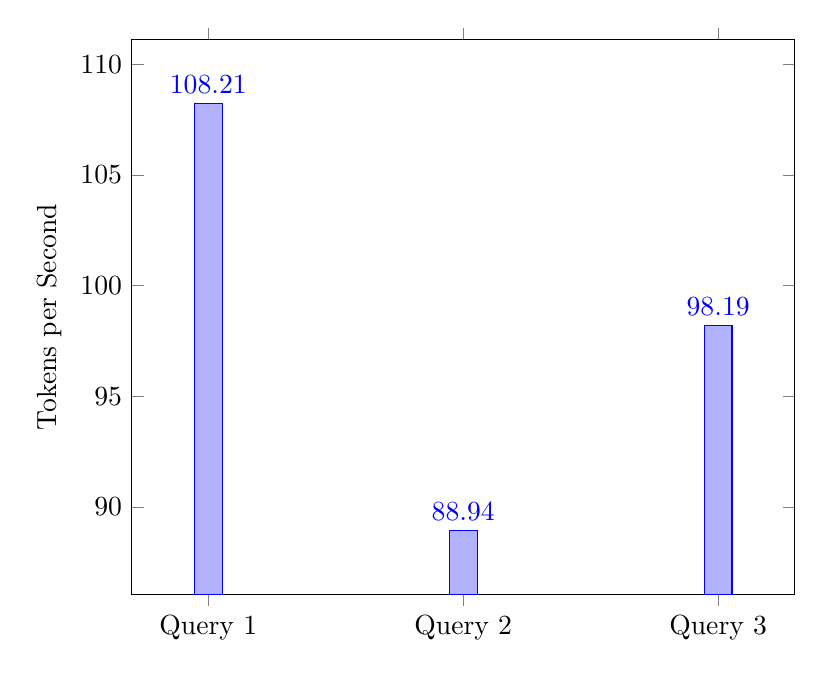
\begin{tikzpicture}
\begin{axis}[
ybar,
enlargelimits=0.15,
legend style={at={(0.5,-0.15)},
anchor=north,legend columns=-1},
ylabel={Tokens per Second},
symbolic x coords={Query 1, Query 2, Query 3},
xtick=data,
nodes near coords,
nodes near coords align={vertical},
]
\addplot coordinates {(Query 1,108.21) (Query 2,88.94) (Query 3,98.19)};
\end{axis}
\end{tikzpicture}
\caption{Token generation throughput (Tokens/Second) for three example test queries.}
\label{fig:throughput}
\end{figure}

I was able to maintain a constant throughput rate of between 88 and 108 tokens-per-second across all three queries, demonstrating the responsiveness of the system to support real-time interactive CLI usage.

\section{Conclusion}

\texttt{ragcli} demonstrates that I have successfully implemented a modern RAG-pipeline as a local CLI-tool without sacrificing performance. By combining the robust vector-search capabilities within Oracle Database 23ai with the lightweight \texttt{gemma3:270m} model, I was able to achieve sub-second retrieval-times and generate new text at rates greater than 90 tokens per second. Future iterations of \texttt{ragcli} will focus on adding re-rankers to improve relevance ranking in addition to improving the ingestion-pipeline for better overall performance.

\end{document}